\documentclass[runningheads,a4paper]{llncs}

\usepackage[utf8]{inputenc}

\usepackage{amssymb}
\setcounter{tocdepth}{3}
\usepackage{graphicx}

\newcommand{\keywords}[1]{\par\addvspace\baselineskip
\noindent\keywordname\enspace\ignorespaces#1}

\usepackage{pifont} 
\usepackage[utf8]{inputenc}
\usepackage{enumitem}
\usepackage[hyphens]{url}
\usepackage[pdftex,urlcolor=black,colorlinks=true,linkcolor=black,citecolor=black]{hyperref}
\def\sectionautorefname{Section}
\def\subsectionautorefname{Subsection}

% listings and Verbatim environment
\usepackage{fancyvrb}
\usepackage{relsize}
\usepackage{listings}
\usepackage{verbatim}
\newcommand{\defaultlistingsize}{\fontsize{8pt}{9.5pt}}
\newcommand{\inlinelistingsize}{\fontsize{8pt}{11pt}}
\newcommand{\smalllistingsize}{\fontsize{6.0pt}{7.0pt}}
\newcommand{\listingsize}{\smalllistingsize}%{\defaultlistingsize}
\RecustomVerbatimCommand{\Verb}{Verb}{fontsize=\inlinelistingsize}
\RecustomVerbatimEnvironment{Verbatim}{Verbatim}{fontsize=\defaultlistingsize}
\lstset{frame=lines,captionpos=b,numberbychapter=false,escapechar=§,
  aboveskip=2em,belowskip=1em,abovecaptionskip=0.5em,belowcaptionskip=0.5em,
  framexbottommargin=-1em,basicstyle=\ttfamily\listingsize\selectfont}

% use Courier from this point onward
\let\oldttdefault\ttdefault
\renewcommand{\ttdefault}{pcr}
\let\oldurl\url
%\renewcommand{\url}[1]{\defaultlistingsize\oldurl{#1}}

\usepackage[usenames,dvipsnames,svgnames,table]{xcolor}
\lstdefinelanguage{JavaScript}{
  keywords={push, typeof, new, true, false, catch, function, return, null,
    catch, switch, var, if, in, while, do, else, case, break, div, script, video},
  keywordstyle=\bfseries,
  ndkeywords={class, export, boolean, throw, implements, import, this},
  ndkeywordstyle=\color{darkgray}\bfseries,
  identifierstyle=\color{black},
  sensitive=false,
  comment=[l]{//},
  morecomment=[s]{/*}{*/},
  morecomment=[s]{<!--}{-->},  
  commentstyle=\color{darkgray},
  stringstyle=\color{green},
  morestring=[b]',
  morestring=[b]"
}
\lstset{breaklines=true}

% linewrap symbol
\usepackage{color}
\definecolor{grey}{RGB}{130,130,130}
\newcommand{\linewrap}{\raisebox{-.6ex}{\textcolor{grey}{$\hookleftarrow$}}}

% todo macro
\usepackage{color}
\newcommand{\todo}[1]{\noindent\textcolor{red}{{\bf \{TODO}: #1{\bf \}}}}

\def\JSONLD{\mbox{JSON-LD}}

\hyphenation{WebVTT}

\def\JSONLD{\mbox{JSON-LD}}

\begin{document}

\mainmatter  % start of an individual contribution

% first the title is needed
\title{Self-Contained Semantic Hypervideos\\ Using Web Components}

% a short form should be given in case it is too long for the running head
\titlerunning{Self-Contained Semantic Hypervideos Using Web Components}

% the name(s) of the author(s) follow(s) next
\author{
  Thomas Steiner\textsuperscript{1}\thanks{Second affiliation: Google, Hamburg, Germany, \email{tomac@google.com}} \and
  Pierre-Antoine Champin\textsuperscript{1} \and \\
  Benoît Encelle\textsuperscript{1}\and
  Yannick Prié\textsuperscript{2}
}
%
\authorrunning{Self-Contained Semantic Hypervideos Using Web Components}
% (feature abused for this document to repeat the title also on left hand pages)

% the affiliations are given next
\institute{
  \textsuperscript{1}CNRS, Université de Lyon, LIRIS -- UMR5205, Université Lyon~1, France\\
  \email{\{tsteiner, pierre-antoine.champin\}@liris.cnrs.fr, benoit.encelle@univ-lyon1.fr}\\
  \textsuperscript{2}CNRS, Université de Nantes, LINA -- UMR 6241, France\\
  \email{yannick.prie@univ-nantes.fr}
}

\maketitle

\begin{abstract}
The creation of hypervideos---displayed video streams
that contain embedded user-clickable anchors and annotations---%
is a~manual and tedious job,
requiring the preparation of assets like still frames,
the segmentation of videos in scenes or chapters,
and sometimes even the isolation of objects
like faces within the video.
In this paper, we propose a~semi-automated
Web-Components-based approach to self-contained hypervideo creation.
By \emph{self-contained} we mean that all necessary intrinsic components
of the hypervideo, \emph{e.g.}, still frames,
should come from the video itself
rather than be included as external assets.
\emph{Web Components} is a~set of specifications,
which let Web developers apply their HTML, CSS,
and JavaScript knowledge to build widgets
that can be reused easily and reliably.
By leveraging this evolving standard,
we obtain a~high degree of abstraction,
which reduces the burden of creating hypervideos
to the familiar task of textually marking them up with HTML elements.

\keywords{Hypervideo, Web Components, semantic video annotation}
\end{abstract}

\section{Introduction}

The term \emph{hypervideo} is commonly used to refer to
\textit{``a~displayed video stream that contains embedded user-clickable anchors''}%
~\cite{sawhney1996hypercafe,smith2002extensible}
and annotations, allowing for navigation between the video and other hypermedia elements.
In a~2006 article in \emph{The Economist}, the authors write 
\textit{``[h]yperlinking video involves the use of ``object-tracking'' software
to make filmed objects, such as cars, clickable as they move around.
Viewers can then click on items of interest in a~video
to watch a related clip; after it has played,
the original video resumes where it left off.
To inform viewers that a~video is hyperlinked,
editors can add highlights to moving images, use beeps as audible cues,
or display still images from hyperlinked videos
next to the clip that is currently playing''}~\cite{economist2006hypervideo}.
In standard literature, hypervideo is considered a~logical consequence
of the related concept of \emph{hypertext}.
In contrast to hypertext, hypervideo necessarily includes a~time component,
as content changes over time.
In consequence, hypervideo has different technical and aesthetic requirements
than hypertext, the most obvious one being appropriate segmentation in scenes
or even objects.
The opportunities for feature-rich semantic hypervideos are endless,
only limited by the feasibility and ease of their creation.
With this paper, we propose an approach that is solely based on 
custom HTML elements that anyone coming from an HTML background can grasp.

\section{Related Work}

Related work can be regarded under the angles
of online video annotation creation and large-scale Linked Data 
efforts for video.
Many have combined Linked Data and video,
typical examples are~\cite{lambert2010linkeddata} by Lambert \emph{et~al.}\
and~\cite{hausenblas2009im} by Hausenblas \emph{et~al.}
There are several text track enriching approaches~\cite{li2013enriching,li2012creating,yi2012synote,steiner2010semwebvid}
based on named entity recognition.
The online video hosting platform YouTube
lets publishers add video annotations
in a~closed proprietary format.
From 2009 to 2010, YouTube had a~feature called
Collaborative Annotations%
~\cite{fink2009collaborativeannotations}
that allowed video consumers to collaboratively
create video annotations.
In~\cite{vandeursen2012mediafragmentannotations},
Van Deursen \emph{et~al.}\ present a~system
that combines Media Fragments URI~\cite{troncy2012mediafragments}
and the Ontology for Media Resources~\cite{lee2012mediaontology}
in an HTML5 Web application to convert
media fragment annotations into a~WebVTT file
that can be used by HTML5-enabled players.
Building on their work, in~\cite{steiner2014webvtt},
we additionally allowed for writing annotations by
letting annotators create WebVTT cues with an editor.
Popcorn.js\footnote{Popcorn.js: \url{http://popcornjs.org/}}
is an HTML5 JavaScript media framework
for the creation of media mixes
by adding interactivity and context to videos
by letting users link social media, feeds,
visualizations, \emph{etc.} to moving images.
PopcornMaker%
\footnote{PopcornMaker: \url{https://popcorn.webmaker.org/}}
is an interactive Web authoring environment
allowing for videos to be annotated on a~timeline.
%Popcorn video annotations are essentially JavaScript~programs.

\section{Web Components}

Web Components is a~set of specifications, which let Web developers leverage
their HTML, CSS, and JavaScript knowledge to build widgets
that can be reused easily and reliably.\footnote{Web Components:
\url{http://www.chromium.org/blink/web-components}}
According to a~(recently discontinued) W3C Working Draft introductory document,%
\footnote{Discontinued W3C Working Draft document:
\url{http://www.w3.org/TR/2013/WD-components-intro-20130606/}}
the component model for the Web (``Web Components'') consists of five pieces:

\begin{description}
  \item[Imports] which defines how templates, decorators and custom elements are packaged and loaded as a~resource.
  \item[Shadow DOM] which encapsulates a~DOM subtree for more reliable composition of user interface elements.    
  \item[Decorators] which apply templates based on CSS selectors to affect rich visual and behavioral changes to documents.
  \item[Custom Elements] which let authors define their own elements, with new tag names and new script interfaces.
  \item[Templates] which define chunks of inert markup that can be activated for use.  
\end{description}

\noindent At time of writing, native support for Web Components
has just landed in a~number of Web browsers,
however, for the majority of browsers,
a~so-called polyfill solution is still required.
A~polyfill  is a~piece of code (or plugin) that provides the technology
that developers expect the browser to provide natively in the near future.
We rely on the Polymer project\footnote{Polymer project:
\url{http://www.polymer-project.org/}}
that provides Web Components support for older browsers.
Polymer allows us to create reusable widgets that introduce a~number of new
custom HTML elements for our task of hypervideo creation.

\section{Implementation Details}

We have developed a~number of Web Components for the creation of hypervideos.
These Web Components are behaviorally grouped together
by a~common naming convention.
In Polymer, all element names have to start with ``polymer-''.

\begin{description}
  \item[\texttt{<polymer-hypervideo>}] is the parent element of all other elements.
    It accepts the attributes \texttt{src} for specifying a~set of
    space-separated video sources (to support different encodings),
    and---analog to the native HTML5 video attributes---%
    \texttt{width} and \texttt{height} for specifying the video's dimensions,
    then \texttt{poster} for specifying the video's poster frame, and finally \texttt{muted} to specify if the video should be initially muted.
  \item[\texttt{<polymer-data-*>}] is a~set of data annotation elements
    that includes the two shorthand annotation types
    \texttt{<polymer-data-actor>} for annotating video actors and
    \texttt{<polymer-data-overlay>} for annotating visual overlays,
    and the generic \texttt{<polymer-data-annotation>} for other annotations.
  \item[\texttt{<polymer-track-*>}] are the two elements
    \texttt{<polymer-track-chapters>} and \texttt{<polymer-track-subtitles>},
    which internally rely on WebVTT~\cite{pfeiffer2013webvtt} text tracks
    of the types ``chapters'' and ``subtitles'' that they enrich with
    automatically generated chapter thumbnails and a~full text subtitle view.
  \item[\texttt{<polymer-visualization-*>}] currently provides the
    following two visualization elements
    \texttt{<polymer-visualization-timeline>} on the one hand and 
    \texttt{<polymer-visualization-toc>} on the other
    that create a~timeline view and a~table of contents
    that put all encountered \texttt{<polymer-track-*>}
    and \texttt{<polymer-data-*>} elements in a~temporal context.
\end{description}

\noindent We make an online demo Web application available at
\url{http://hypervideo.herokuapp.com} and also share its source code.%
\footnote{Hypervideo Demo:
\url{https://github.com/tomayac/postdoc/tree/master/demos/polymer-hypervideo}}
As both native Web Component support in Web browsers and the Polymer project
are constantly evolving and still in flux, the demo currently works best on
Opera v22.0.1471.70	(Mac~OS~X).
A~screenshot of the application can be seen in \autoref{fig:screenshot},
the corresponding underlying code sample is shown in \autoref{listing:polymer}.
These components communicate with each other through standard JavaScript events,
so when a~components needs to communicate its state to another, \emph{e.g.},
\texttt{<polymer-hypervideo>} the current time of the video to one of the
visualization components like the \texttt{<polymer-visualization-timeline>},
it fires an event that components can subscribe to and react upon.
\autoref{listing:events} shows the relevant code snippets.

\begin{lstlisting}[caption={Web Components mark-up for the hypervideo in \autoref{fig:screenshot}, including subtitles, chapters, timeline, and table of contents widgets; the actor annotation contains a spatial fragment
(\texttt{xywh})~\cite{troncy2012mediafragments} and a~hyperlink (\texttt{url})
  to Wikimedia Commons},
  label=listing:polymer, language=xml,
  float=b!, stringstyle=\color{gray},morekeywords={polymer,hypervideo,track,subtitles,chapters,toc,timeline,visualization,data,actor,src,end,start,name,url,width,height,muted,displaysubtitlesgroup,orientation,displaychaptersthumbnails,xywh}]
<polymer-hypervideo src="big_buck_bunny.mp4 big_buck_bunny.webm" width="400" height="225" muted>
  <polymer-data-actor start="10" end="35" name="Chirp (Owl)" xywh="170,20,70,80" 
      url="http://commons.m.wikimedia.org/wiki/File:Chirp1_-_BBB_-_reduced_snapshot.png">
  </polymer-data-actor>
  <polymer-track-subtitles src="subtitles.vtt" displaysubtitlesgroup></polymer-track-subtitles>
  <polymer-track-chapters src="thumbs.vtt" displaychaptersthumbnails></polymer-track-chapters>
  <polymer-visualization-timeline orientation="landscape"></polymer-visualization-timeline>
  <polymer-visualization-toc></polymer-visualization-toc>
</polymer-hypervideo>
\end{lstlisting}

\begin{lstlisting}[caption={Native JavaScript event communication
  between Web Components},
  label=listing:events, language=JavaScript,
  float=b!, stringstyle=\color{gray},morekeywords={addEventListener,document}]
// === In polymer-hypervideo.js: ===
// listen to native html5 video timeupdate events
video.addEventListener('timeupdate', function() {
  that.currentTime = video.currentTime;
  // publish hypervideotimeupdate events
  that.fire('hypervideotimeupdate', { currentTime: that.currentTime });
});

// === In polymer-visualization-timeline.js: ===
// listen to hypervideotimeupdate events
document.addEventListener('hypervideotimeupdate', function(e) {
  var currentTime = e.detail.currentTime;
  // update the time marker
});
\end{lstlisting}

\begin{figure}[hbt]
  \centering
  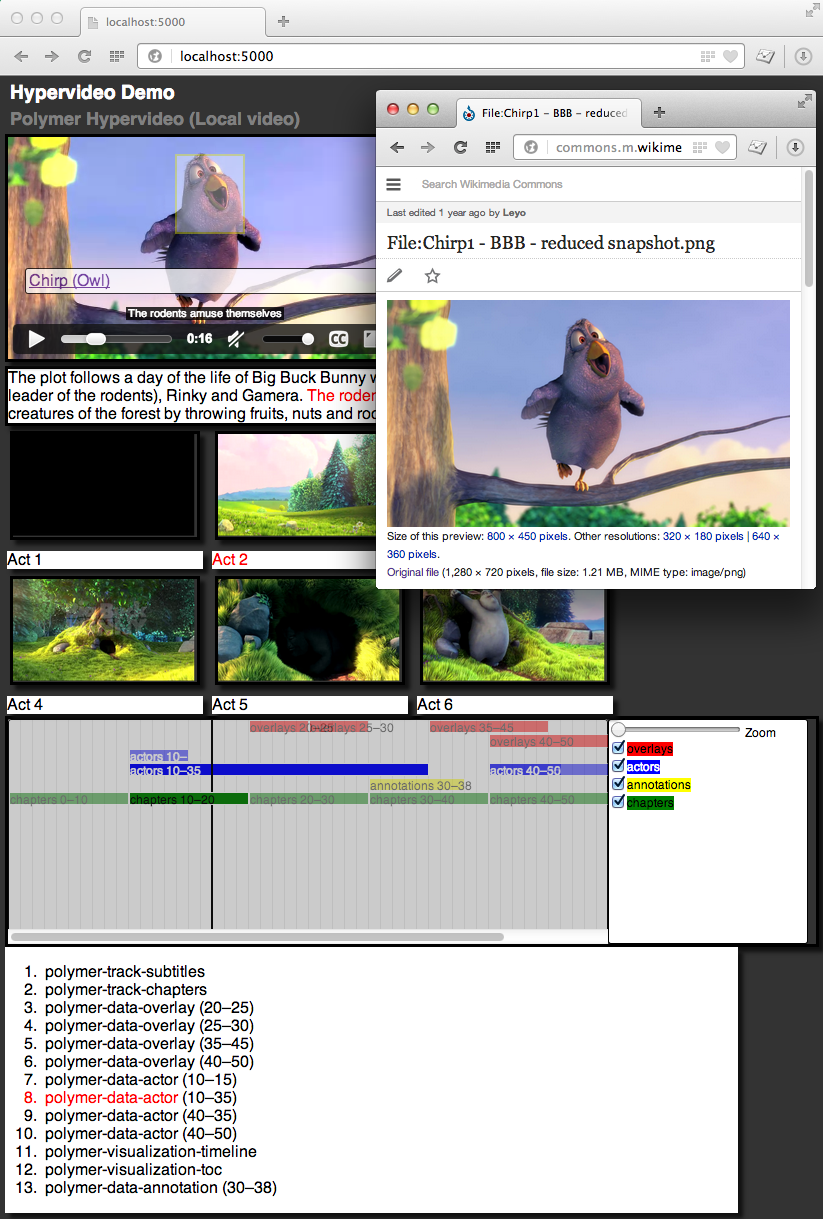
\includegraphics[width=0.575\linewidth]{screenshot}
  \caption{Generated hypervideo based on the mark-up in \autoref{listing:polymer},
  including subtitles, chapters, timeline, and table of contents widgets;
  the actor annotation contains a spatial fragment~\cite{troncy2012mediafragments}
  (owl's head) and a~hyperlink
  to a~details page on Wikimedia Commons}
  \label{fig:screenshot}
\end{figure}

\section{Linked Data Considerations}

``As Polymer makes use of polyfills, search engines treat Polymer-based
applications no differently than they do other JavaScript-based Web apps.
In fact, Google’s crawler understands JavaScript heavy applications.%
\footnote{Google Web application understanding:
\url{http://googlewebmastercentral.blogspot.com/2014/05/understanding-web-pages-better.html}}
Going forward, it is a~reasonable assumption
that as use of native Shadow DOM increases,
search engine providers will try to adapt to understand it,
just as they have adapted to other new Web technologies in the past.''%
\footnote{From the FAQ of Polymer:
\url{http://www.polymer-project.org/resources/faq.html}}
In the longterm, this paths the way toward the semantic information
introduced through Web Components mark-up
not being lost by search engines and Linked Data crawlers,
but being understood.

\section{Conclusions and Future Work}

In this paper, we have introduced a~Web-Components-based approach
for the generation of hypervideos with nothing more than custom HTML elements.
We have made both a~demo application and the underlying source code
as well as the source code of the mentioned Web Components available.
Immediate next steps are to improve the browser compatibility
and to migrate the code to the native Web Components implementation
that will soon be encountered in all major Web browsers.
Concluding, Web Components radically redefine how we develop applications
on the Web.
With our code, we have shown that this certainly holds true for hypervideo
and are excited about future applications and use cases.

\bibliographystyle{abbrv}
\bibliography{references}
\end{document}
